\section{Main theorem}
\newcommand{\Xij}{X_{ij}}
\newcommand{\Xji}{X_{ji}}
\newcommand{\Tij}{T_{ij}}
\newcommand{\Tji}{T_{ji}}
\newcommand{\sij}{\sigma_{ij}}
\newcommand{\sji}{\sigma_{ji}}
\newcommand{\rij}{\rho_{ij}}
\newcommand{\rji}{\rho_{ji}}
\newcommand{\dotcirc}{+}
\newcommand{\bigdotcirc}{\sum}

\begin{frame}{Simplifying swirling}
Swirling involves concatenating dependent paths. Can we simplify that?
\end{frame}

\begin{frame}{Pay off all our assumptions 1: torsor structure, vector field}
\begin{columns}
\begin{column}{0.15\textwidth}
\begin{tikzcd}[ampersand replacement=\&, column sep=small]
  {T_1} \\
  {T_{13}T_{32}T_{21}X_1} \\
  {T_{13}T_{32}X_2} \\
  {T_{13}X_3} \\
  {X_1}
  \arrow["{\alert{T_{13}T_{32}X_{21}}:}", equals, from=3-1, to=2-1]
  \arrow["{\alert{T_{13}X_{32}}:}", equals, from=4-1, to=3-1]
  \arrow["{\alert{X_{13}}:}", equals, from=5-1, to=4-1]
\end{tikzcd}

\end{column}
\begin{column}{0.85\textwidth}
\begin{itemize}
\item<2-> Def: \( \alpha_i\defeq s(-,X_i):T_i\simto S^1 \) (\alert{trivialization on 0-skeleton}).
\item<3-> Def: \( \rji\defeq \alpha_j(\Tji(X_i)) \) is \alert{the rotation of \( \Tji \)}.
% https://q.uiver.app/#q=WzAsNCxbMCwwLCJUX2kiXSxbMSwwLCJUX2oiXSxbMCwxLCJTXjEiXSxbMSwxLCJTXjEiXSxbMCwxLCJUX3tqaX0iXSxbMCwyLCJcXGFscGhhX2kiLDJdLFsxLDMsIlxcYWxwaGFfaiJdLFsyLDMsIigtKVxcY2RvdFxccmhvX3tqaX0iLDJdLFszLDEsIlxcbWF0aHNme2Jhc2V9XFxtYXBzdG8gWF9qIiwyLHsib2Zmc2V0IjozLCJjdXJ2ZSI6MX1dLFsyLDAsIlxcbWF0aHNme2Jhc2V9XFxtYXBzdG8gWF9pIiwwLHsib2Zmc2V0IjotMywiY3VydmUiOi0xfV1d
\[\begin{tikzcd}[ampersand replacement=\&]
  {T_i} \& {T_j} \\
  {S^1} \& {S^1}
  \arrow["{T_{ji}}", from=1-1, to=1-2]
  \arrow["{\alpha_i}"', from=1-1, to=2-1]
  \arrow["{\alpha_j}", from=1-2, to=2-2]
  \arrow["{\mathsf{base}\mapsto X_i}", shift left=3, curve={height=-6pt}, from=2-1, to=1-1]
  \arrow["{(-)\dotcirc\rho_{ji}}"', from=2-1, to=2-2]
  \arrow["{\mathsf{base}\mapsto X_j}"', shift right=3, curve={height=6pt}, from=2-2, to=1-2]
\end{tikzcd}\]
\item<4-> Lemma: \( \rij=\rji^{-1} \) because \alert{in \( T_j \)}: \( \rij\dotcirc\rji\dotcirc X_j=\rij\dotcirc \Tji X_i=\Tji(\rij\dotcirc X_i)=\Tji \Tij X_j=X_j \).
\end{itemize}
\end{column}
\end{columns}
\end{frame}

\begin{frame}{Pay off all our assumptions 1: torsor structure, vector field (cont.)}
\begin{columns}
\begin{column}{0.15\textwidth}
\begin{tikzcd}[ampersand replacement=\&, column sep=small]
  {T_1} \\
  {T_{13}T_{32}T_{21}X_1} \\
  {T_{13}T_{32}X_2} \\
  {T_{13}X_3} \\
  {X_1}
  \arrow["{\alert{T_{13}T_{32}X_{21}}:}", equals, from=3-1, to=2-1]
  \arrow["{\alert{T_{13}X_{32}}:}", equals, from=4-1, to=3-1]
  \arrow["{\alert{X_{13}}:}", equals, from=5-1, to=4-1]
\end{tikzcd}

\end{column}
\begin{column}{0.5\textwidth}
\begin{itemize}
\item<2-> Define \( \sji\defeq \alpha_j(\Xji):\rji=_{S^1}\base, \).
\item<3-> Paths of the form \( (a=_{S^1}\base) \) can be multiplied: 
\begin{itemize}
\item \( \dotcirc:(a=\base)\times (b=base)\to (a\dotcirc b=base) \).
\item \( p\dotcirc q=(p\dotcirc b)\cdot q. \)
\end{itemize}
\item<4-> Lemma: \( \apd(X)(\refl)=\refl\) \(\implies \Xij\cdot \Tij\Xji=\refl_{X_i}\) \(\implies\sij\dotcirc\sji=\refl_{\base} \) (\( \Tij \) just translates \( \Xji \) to cat with \( \Xji \)).
\end{itemize}
\end{column}
\begin{column}{0.35\textwidth}
\onslide<5->{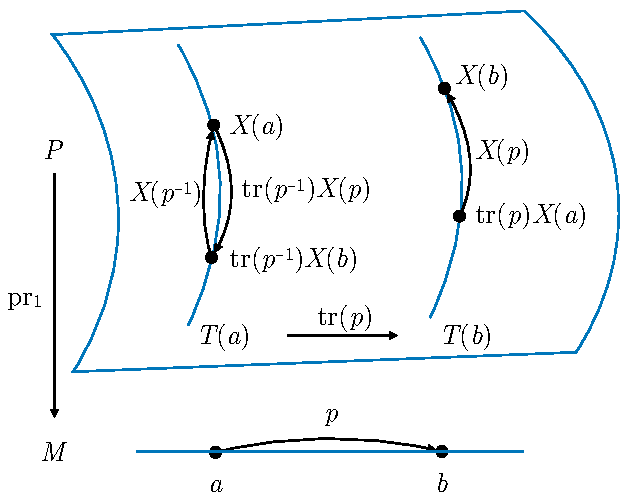
\includegraphics[width=30ex]{figs/pathovers_inverse.pdf}}
\end{column}
\end{columns}
\end{frame}

\begin{frame}{Pay off all our assumptions 2: no boundary, commutativity}
\begin{columns}
\begin{column}{0.15\textwidth}
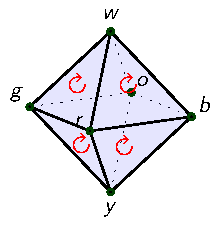
\includegraphics{figs/oo_orientation.pdf}
\end{column}
\begin{column}{0.85\textwidth}
\begin{mydef}
Let \( F_1,\ldots,F_n \) be the faces of \( \mm \), \( v_i:F_i \) be designated vertices, and \( \partial F_i:v_i=v_i \) be the triangular boundaries. The \alert{total swirling} is \[ X_\tot \defeq \sigma_{\partial F_1}\dotcirc\cdots\dotcirc\sigma_{\partial F_n} \].
\end{mydef}
\begin{itemize}
\item<2-> We assume that this expression involves \alert{every edge once in each direction}.
\item<3-> \( S^1 \) is commutative, hence \alert{complete cancellation}.
\end{itemize}
\end{column}
\end{columns}
\end{frame}

\begin{frame}{Consequence}
\vspace{-6ex}
\[\begin{aligned}
\tr_F&\defeq \tr(\partial F)&&:T_1=_{BS^1}T_1&&\text{\alert{curvature}}\\
\flat_F&\defeq \flat(\partial F)&&:\id=_{(T_1=_{BS^1}T_1)}\tr_F&&\text{\alert{flatness}}\\
X_F&\defeq X(\partial F)&&:\tr_F(X_1)=_{T_1}X_1&&\text{\alert{swirling}}\\
L^X_F&\defeq\flat_F(X_1)\cdot X_F&&:(X_1=_{T_1}X_1)&&\text{\alert{flattened swirling}}
\end{aligned}\]
\onslide<2->{
These can all be totaled in \( S^1 \) to give
\begin{columns}[t]
\begin{column}{0.5\textwidth}
\[\begin{aligned}
\tr_\tot&\defeq \bigdotcirc_i \rho_{\partial F} = \base\\
\flat_\tot&\defeq \bigdotcirc_i\flat_{\partial F}\\
\end{aligned}\]
\end{column}
\begin{column}{0.5\textwidth}
\[\begin{aligned}
X_\tot&\defeq \bigdotcirc_i \sigma_{\partial F} = \refl_\base\\
L^X_\tot&\defeq \bigdotcirc_i \flat_{\partial F} \dotcirc \sigma_{\partial F} = \bigdotcirc_i \flat_{\partial F}
\end{aligned}\]
\end{column}
\end{columns}
}\onslide<3->{
So in our lingo: the total flatness equals the total flattened swirling.\qed
}
\end{frame}

\begin{frame}{Examples}
\tikzset{every picture/.style={scale=0.65}}
\[\begin{figure}[h]
\centering
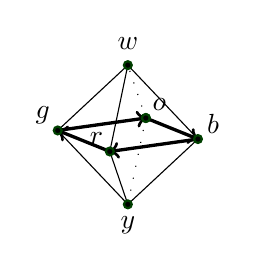
\begin{tikzpicture}%
  [x={(-0.860769cm, -0.121512cm)},
  y={(0.508996cm, -0.205391cm)},
  z={(-0.000053cm, 0.971107cm)},
  scale=1,
  eqback/.style={->, very thick},
  back/.style={loosely dotted, thin},
  eqedge/.style={->, very thick},
  edge/.style={black, thin},
  facet/.style={fill=blue!95!black,fill opacity=0.0},
  vertex/.style={inner sep=1pt,circle,draw=green!25!black,fill=black,thick}]
\coordinate (-1, -1, 0) at (-1, -1, 0);
\coordinate (-1, 1, 0) at (-1, 1, 0);
\coordinate (0, 0, -1) at (0, 0, -1);
\coordinate (0, 0, 1) at (0, 0, 1);
\coordinate (1, -1, 0) at (1, -1, 0);
\coordinate (1, 1, 0) at (1, 1, 0);
%% Drawing edges in the back
%%
\draw[edge,eqback] (-1, -1, 0) -- (-1, 1, 0);
\draw[edge,back] (-1, -1, 0) -- (0, 0, -1.4);
\draw[edge,back] (-1, -1, 0) -- (0, 0, 1.4);
\draw[edge,eqback] (1, -1, 0) -- (-1, -1, 0);
%% Drawing vertices in the back
%%
\node[vertex] at (-1, -1, 0)     {};
%% Drawing the facets
%%
\fill[facet] (1, 1, 0) -- (0, 0, -1.4) -- (1, -1, 0) -- cycle {};
\fill[facet] (1, 1, 0) -- (0, 0, 1.4) -- (1, -1, 0) -- cycle {};
\fill[facet] (1, 1, 0) -- (-1, 1, 0) -- (0, 0, 1.4) -- cycle {};
\fill[facet] (1, 1, 0) -- (-1, 1, 0) -- (0, 0, -1.4) -- cycle {};
%% Drawing edges in the front
%%
\draw[edge] (-1, 1, 0) -- (0, 0, -1.4);
\draw[edge] (-1, 1, 0) -- (0, 0, 1.4);
\draw[eqedge] (-1, 1, 0) -- (1, 1, 0);
\draw[edge] (0, 0, -1.4) -- (1, -1, 0);
\draw[edge] (0, 0, -1.4) -- (1, 1, 0);
\draw[edge] (0, 0, 1.4) -- (1, -1, 0);
\draw[edge] (0, 0, 1.4) -- (1, 1, 0);
\draw[eqedge] (1, 1, 0) -- (1, -1, 0);
%% Drawing the vertices in the front
%%
\begin{scope}[nodes=vertex]
\node[label=above right:\( b \)] at (-1, 1, 0)     {};
\node[label=below:\( y \)] at (0, 0, -1.4)     {};
\node[label=above:\( w \)] at (0, 0, 1.4)     {};
\node[label=above left:\( g \)] at (1, -1, 0)     {};
\node[label=above left:\( r \)] at (1, 1, 0)     {};
\node[label=above right:\( o \)] at (-1, -1, 0)     {};
\end{scope}
\end{tikzpicture}

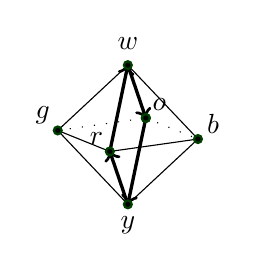
\begin{tikzpicture}%
  [x={(-0.860769cm, -0.121512cm)},
  y={(0.508996cm, -0.205391cm)},
  z={(-0.000053cm, 0.971107cm)},
  scale=1,
  eqback/.style={->, very thick},
  back/.style={loosely dotted, thin},
  eqedge/.style={->, very thick},
  edge/.style={black, thin},
  facet/.style={fill=blue!95!black,fill opacity=0.0},
  vertex/.style={inner sep=1pt,circle,draw=green!25!black,fill=black,thick}]
\coordinate (-1, -1, 0) at (-1, -1, 0);
\coordinate (-1, 1, 0) at (-1, 1, 0);
\coordinate (0, 0, -1) at (0, 0, -1);
\coordinate (0, 0, 1) at (0, 0, 1);
\coordinate (1, -1, 0) at (1, -1, 0);
\coordinate (1, 1, 0) at (1, 1, 0);
%% Drawing edges in the back
%%
\draw[edge,back] (-1, -1, 0) -- (-1, 1, 0);
\draw[edge,eqback] (-1, -1, 0) -- (0, 0, -1.4);
\draw[edge,eqback] (0, 0, 1.4) -- (-1, -1, 0);
\draw[edge,back] (1, -1, 0) -- (-1, -1, 0);
%% Drawing vertices in the back
%%
\node[vertex] at (-1, -1, 0)     {};
%% Drawing the facets
%%
\fill[facet] (1, 1, 0) -- (0, 0, -1.4) -- (1, -1, 0) -- cycle {};
\fill[facet] (1, 1, 0) -- (0, 0, 1.4) -- (1, -1, 0) -- cycle {};
\fill[facet] (1, 1, 0) -- (-1, 1, 0) -- (0, 0, 1.4) -- cycle {};
\fill[facet] (1, 1, 0) -- (-1, 1, 0) -- (0, 0, -1.4) -- cycle {};
%% Drawing edges in the front
%%
\draw[edge] (-1, 1, 0) -- (0, 0, -1.4);
\draw[edge] (-1, 1, 0) -- (0, 0, 1.4);
\draw[edge] (-1, 1, 0) -- (1, 1, 0);
\draw[edge] (0, 0, -1.4) -- (1, -1, 0);
\draw[eqedge] (0, 0, -1.4) -- (1, 1, 0);
\draw[edge] (0, 0, 1.4) -- (1, -1, 0);
\draw[eqedge] (1, 1, 0) -- (0, 0, 1.4) ;
\draw[edge] (1, 1, 0) -- (1, -1, 0);
%% Drawing the vertices in the front
%%
\begin{scope}[nodes=vertex]
\node[label=above right:\( b \)] at (-1, 1, 0)     {};
\node[label=below:\( y \)] at (0, 0, -1.4)     {};
\node[label=above:\( w \)] at (0, 0, 1.4)     {};
\node[label=above left:\( g \)] at (1, -1, 0)     {};
\node[label=above left:\( r \)] at (1, 1, 0)     {};
\node[label=above right:\( o \)] at (-1, -1, 0)     {};
\end{scope}
\end{tikzpicture}

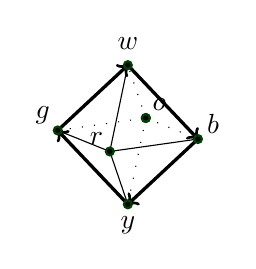
\begin{tikzpicture}%
  [x={(-0.860769cm, -0.121512cm)},
  y={(0.508996cm, -0.205391cm)},
  z={(-0.000053cm, 0.971107cm)},
  scale=1,
  eqback/.style={->, very thick},
  back/.style={loosely dotted, thin},
  eqedge/.style={->, very thick},
  edge/.style={black, thin},
  facet/.style={fill=blue!95!black,fill opacity=0.0},
  vertex/.style={inner sep=1pt,circle,draw=green!25!black,fill=black,thick}]
\coordinate (-1, -1, 0) at (-1, -1, 0);
\coordinate (-1, 1, 0) at (-1, 1, 0);
\coordinate (0, 0, -1) at (0, 0, -1);
\coordinate (0, 0, 1) at (0, 0, 1);
\coordinate (1, -1, 0) at (1, -1, 0);
\coordinate (1, 1, 0) at (1, 1, 0);
%% Drawing edges in the back
%%
\draw[edge,back] (-1, -1, 0) -- (-1, 1, 0);
\draw[edge,back] (-1, -1, 0) -- (0, 0, -1.4);
\draw[edge,back] (-1, -1, 0) -- (0, 0, 1.4);
\draw[edge,back] (1, -1, 0) -- (-1, -1, 0);
%% Drawing vertices in the back
%%
\node[vertex] at (-1, -1, 0)     {};
%% Drawing the facets
%%
\fill[facet] (1, 1, 0) -- (0, 0, -1.4) -- (1, -1, 0) -- cycle {};
\fill[facet] (1, 1, 0) -- (0, 0, 1.4) -- (1, -1, 0) -- cycle {};
\fill[facet] (1, 1, 0) -- (-1, 1, 0) -- (0, 0, 1.4) -- cycle {};
\fill[facet] (1, 1, 0) -- (-1, 1, 0) -- (0, 0, -1.4) -- cycle {};
%% Drawing edges in the front
%%
\draw[eqedge] (-1, 1, 0) -- (0, 0, -1.4);
\draw[eqedge] (0, 0, 1.4) -- (-1, 1, 0);
\draw[edge] (-1, 1, 0) -- (1, 1, 0);
\draw[eqedge] (0, 0, -1.4) -- (1, -1, 0);
\draw[edge] (0, 0, -1.4) -- (1, 1, 0);
\draw[eqedge] (1, -1, 0) -- (0, 0, 1.4);
\draw[edge] (0, 0, 1.4) -- (1, 1, 0);
\draw[edge] (1, 1, 0) -- (1, -1, 0);
%% Drawing the vertices in the front
%%
\begin{scope}[nodes=vertex]
\node[label=above right:\( b \)] at (-1, 1, 0)     {};
\node[label=below:\( y \)] at (0, 0, -1.4)     {};
\node[label=above:\( w \)] at (0, 0, 1.4)     {};
\node[label=above left:\( g \)] at (1, -1, 0)     {};
\node[label=above left:\( r \)] at (1, 1, 0)     {};
\node[label=above right:\( o \)] at (-1, -1, 0)     {};
\end{scope}
\end{tikzpicture}
\caption{The equators for \( w, b, r \).}
\end{figure}\]
Each face contributes \( \flat_F=H_R \), a 1/4-rotation. Total: 2.
\onslide<2->{
\begin{columns}
\begin{column}{0.2\textwidth}
\begin{tikzpicture}%
  [x={(-0.860769cm, -0.121512cm)},
  y={(0.508996cm, -0.205391cm)},
  z={(-0.000053cm, 0.971107cm)},
  scale=1,
  back/.style={loosely dotted, thin},
  edge/.style={black, thick},
  arrow/.style={black, very thick, solid, -{Stealth[scale=0.8]}},
  facet/.style={fill=blue!95!black,fill opacity=0.0},
  vertex/.style={inner sep=1pt,circle,draw=green!25!black,fill=black,thick}]
%% Drawing the vertices in the front
%%
\begin{scope}[nodes=vertex]
\node[label=above right:\( b \)] at (-1, 1, 0) (b)     {};
\node[label=below:\( y \)] at (0, 0, -1.4) (y)    {};
\node[label=above:\( w \)] at (0, 0, 1.4)  (w)   {};
\node[label=above left:\( g \)] at (1, -1, 0) (g)    {};
\node[label=above left:\( r \)] at (1, 1, 0)  (r)   {};
\node[label=above right:\( o \)] at (-1, -1, 0) (o)    {};
\end{scope}
%% Drawing edges in the back
%%
\draw[edge,back,arrow] (o) -- (b);
\draw[edge,back,arrow] (y) -- (o);
\draw[edge,back] (o) -- (w);
\draw[edge,back] (o) -- (g);
%% Drawing vertices in the back
%%
\node[vertex] at (o)     {};
%% Drawing the facets
%%
\fill[facet] (1, 1, 0) -- (0, 0, -1.4) -- (1, -1, 0) -- cycle {};
\fill[facet] (1, 1, 0) -- (0, 0, 1.4) -- (1, -1, 0) -- cycle {};
\fill[facet] (1, 1, 0) -- (-1, 1, 0) -- (0, 0, 1.4) -- cycle {};
\fill[facet] (1, 1, 0) -- (-1, 1, 0) -- (0, 0, -1.4) -- cycle {};
%% Drawing edges in the front
%%
\draw[edge,arrow] (b) -- (y);
\draw[edge] (b) -- (w);
\draw[edge] (b) -- (r);
\draw[edge] (y) -- (g);
\draw[edge] (y) -- (r);
\draw[edge,arrow] (g) -- (w);
\draw[edge,arrow] (w) -- (r);
\draw[edge,arrow] (r) -- (g);
\end{tikzpicture}

\end{column}
\begin{column}{0.8\textwidth}
This is what it looks like: +1 from \( F_{wrg} \), +1 from \( F_{ybo} \), +0 from others.
\end{column}
\end{columns}}
\end{frame}

\begin{frame}{Classical proof}
\begin{columns}
\column{0.5\textwidth}
\vspace{12pt}
\begin{figure}
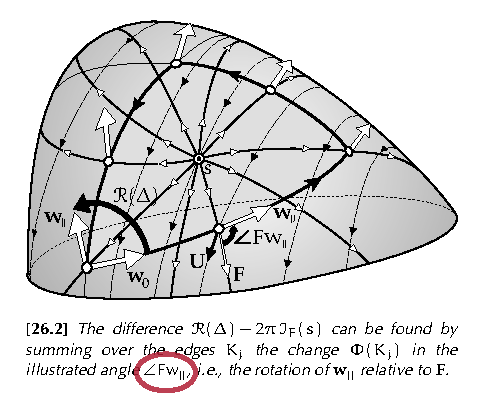
\includegraphics[width=0.9\textwidth]{figs/needham_triangle_circ.pdf}
\caption{{Needham,~T. (2021) Visual Differential Geometry and Forms.}}
\end{figure}
\column{0.5\textwidth}
\vspace{-12pt}
\begin{itemize}
\item The classical proof is discrete-flavored.
\item ``\( \angle Fw_{||} \)'' looked a lot like a pathover.
\item Hopf's \( \Phi \) is defined on edges, not loops. We imitated that too.
\end{itemize}
\end{columns}
\end{frame}
